\subsection{Временное разрешение}

В проведенных пучковых тестах имеют место два типа событий, в которых регистрируется несколько практически одновременно испущенных фотонов. Первый тип – это вспышка лазера, длительность которой на порядок меньше разброса времени прохождения сигнала через МАФЭУ. Второй тип – черенковские кольца. В этом случае разброс времен прихода фотонов на МАФЭУ не превышает 1 пс (Егор, вы прикидывали геометрию, там 1пс или «единицы пикосекунд?»). Анализ таких событий позволяет охарактеризовать временное разрешение всей системы считывания, начиная от окна МАФЭУ и кончая генерацией отметок времени. Временное разрешение одного канала определяется разбросом зарегистрированных временных отметок относительно времени прилета фотона при многократных измерениях. Поскольку точное время прилета фотона измерить нельзя, нам приходится исследовать разброс разностей временных отметок в паре каналов при регистрации одновременно пришедших фотонов. Временные отметки в каждом из каналов подвержены независимым флуктуациям по одинаковому закону, следовательно, измеренная ширина распределения будет в $ \sqrt(2) $ раз больше, чем временно разрешение каждого канала. Типичное распределение разностей временных отметок, принадлежащих одной вспышке лазера, после применения коррекций задержек и калибровки точного времени в двух каналах, ни один из которых не является дефектным, показано на рис. \ref{fig:TimeRes}.

\begin{figure}
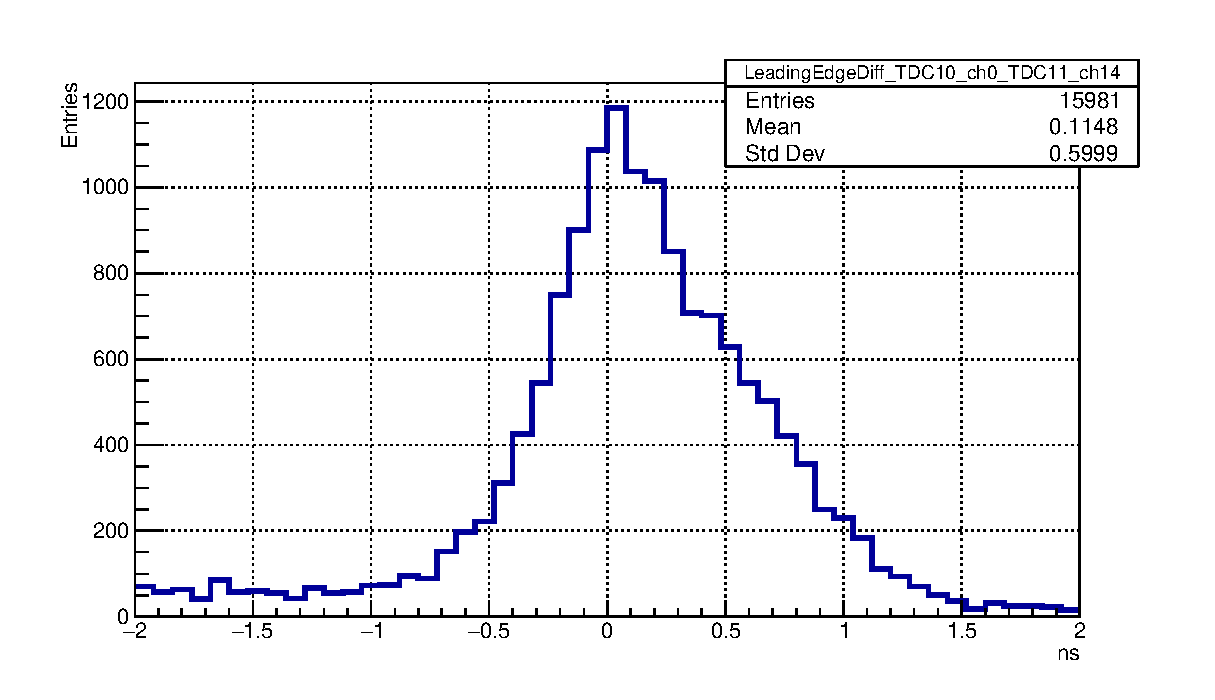
\includegraphics[width=1.0\textwidth]{pictures/LeadingEdgeDiff_TDC10_ch0_TDC11_ch14_corr.eps}
\caption{Распределение разности временных отметок передних фронтов, соответствующих фотонам из одной вспышки лазера, зарегистрированных в заданной паре каналов после применения калибровки точного времени и коррекции задержек.}
\label{fig:TimeRes}
\end{figure}

Полная ширина на полувысоте этого распределения составляет ??? пс, что соответствует временному разрешению ??? пс. Данное значение превосходит разброс времен прохождения сигнала в МА~ФЭУ примерно в 2 раза. Причина расхождения заключается в отсутствии коррекции момента пересечения порога в зависимости от амплитуды сигнала. Для реализации такой коррекции необходимо надежное измерение времени над порогом, что в нашем случае невозможно, см. пункт ???.

Для того чтобы охарактеризовать временное ???измерение??? (разрешение?) системы в целом, помимо анализа пар каналов исследовались физически одновременные сигналы на следующих совокупностях каналов: (1) шестнадцать каналов, считываемых одной платой PADIWA, (2) 64 канала, принадлежащих одному МАФЭУ, (3) 256 каналов, принадлежащих четырем соседним МАФЭУ. В каждом случае после коррекции задержек и калибровки точного времени, отбирались все хиты, принадлежащие одному событию и гистограммировались разности временных отметок по всем возможным парам каналов. Результаты для вспышек лазера показаны на рис \ref{fig:TimeResEvolutionLaser}. В таблице \ref{} показано, как эволюционирует среднеквадраттичное отклонение и полная ширина на полувысоте (FWHM) в зависимости от числа каналов. Отметим, что среднеквадратичное отклонение меняется слабо, а FWHM возрастает с увеличением числа каналов, одновременно с тем, что распределение принимает форму последовательно (передвинуть слово?) более близкую к распределению Гаусса. Такое поведение можно интерпретировать как размывание индивидуальнх особенностей каналов в процессе усреднения. Аналогичное поведение наблюдается и для хитов, принадлежащих одному черенковскому кольцу, см. рис. \ref{fig:TimeResEvolutionRings}. Наблюдаемое смещение максимума от нуля можно объяснить, а можно и не объяснять.

\begin{figure}
\label{fig:TimeResEvolutionLaser}
\end{figure}


\begin{figure}
\label{fig:TimeResEvolutionRings}
\end{figure}